%% ===================================================================
\section{Background}
\label{sec:background}
%% ===================================================================

In the differentiable symbolic regression variant studied here, a
fixed binary tree of operator nodes is parameterized so that
gradient descent learns the leaf weights and a soft selection of
the input that each internal node receives.  An architecture
specifies the tree's depth, branching pattern, and the routing of
input variables through the tree.

The EML operator~\citep{Odrzywolek2026eml} is the binary
expression $\eml(a,b) = e^a - \ln b$.  Setting one argument to a
constant exposes one half: $\eml(x,1) = e^x$ and
$\eml(0,x) = 1 - \ln x$.  The two halves can also be exercised
at once, as in $\eml(x,x) = e^x - \ln x$ or
$\eml(\eml(x,1),\,x) = e^{e^x} - \ln x$.  With the constant~$1$
available at leaves, EML has been proposed as a functionally
complete operator for elementary
expressions~\citep{Odrzywolek2026eml}.  In this paper, however,
the relevant question is narrower, whether the tested depth-3
targets are representable and recoverable under training and
hardening.  Although the cited operator has broad expressivity
in principle, the experiments here are depth-limited.  The
relevant question is therefore whether a target lies inside the
hardened depth-3 architecture and whether training can recover
that target.

The two arguments of $\eml$ have asymmetric partial derivatives:
$\partial\eml/\partial a = e^a$ grows exponentially with $a$,
while $\partial\eml/\partial b = -1/b$ shrinks toward zero as
$b$ grows.  By the chain rule, the gradient of the training MSE
at any parameter is the product of local derivatives along the
path from that parameter to the root.  In the observed training
regime, many internal outputs exceed one.  In that regime, a
path through more left-side ($a$) inputs accumulates
amplification, while a path through more right-side ($b$) inputs
accumulates attenuation.  Routing a variable through more
left-side inputs is therefore expected to increase its gradient
magnitude relative to right-side routing.

A binary tree of depth~$n$ has $2^n - 1$ internal nodes and
$2^n$ leaves.  Depth~3 gives seven internal nodes and eight leaves,
the template used throughout this study.  Each internal node is
given a small set of candidate inputs, and training selects one of
them, so different selections collapse the same template into
different \emph{active} subtrees.  Many active subtrees are
admissible at depth~3; this study focuses on five archetypal
shapes that span the chain and balanced extremes
(Fig.~\ref{fig:topologies}).  Four are chains: at each internal
level above the deepest, one branch continues into a subtree
while the other reduces to the constant~1; the deepest active
node takes the variable leaves $x$ and $y$.  Chain shapes are labeled by which $\eml$
argument carries the active branch at the root and at depth~1,
left ($a$) or right ($b$), giving LR, RL, RR, and LL.

The fifth is balanced.  Both root children are $\eml$ nodes that
take leaves directly, so its active subtree occupies only the top
two levels of the depth-3 template.  The LL chain produces triply iterated
exponentiation ($e^{e^{e^x}}$ at unit-leaf inputs), which
overflows on the training domain and is excluded from experiments.

All three architectures share the depth-3 template and differ
only in how each internal node selects its inputs
(Table~\ref{tab:archs}); each contains every target in this paper
inside its representable set.  Eq.\,6 is taken directly from
Eq.~(6) of~\citet{Odrzywolek2026eml}: a softmax at every internal
node selects among $\{1, x, f_{\text{child}}\}$, where
$f_{\text{child}}$ at each input position denotes the output of
the $\eml$ subtree rooted at that position, so the variable~$x$
can enter at every level but $y$ enters only at the leaves.  V16
is variant~16 of the EML reference implementation released with
the cited paper~\citep{Odrzywolek2026eml}: a
sigmoid at every internal node selects between
$\{1, f_{\text{child}}\}$, and $x$ and $y$ enter only at the
leaves through a three-way softmax over $\{x, y, 1\}$, treating
the two variables symmetrically.  These two architectures differ
in two ways at once.  They have different selector arity (softmax over three inputs
versus sigmoid over two) and different variable-routing asymmetry
(favoring~$x$ versus treating $x,y$ alike).  Hybrid localizes
this distinction to the root.  Hybrid uses V16's sigmoid at
every internal node other than the root, where a four-way
softmax additionally admits $x$ and $y$, granting both variables
direct root access without otherwise altering the V16 selector
pattern.

\begin{figure}[t]
\centering
\resizebox{\columnwidth}{!}{%
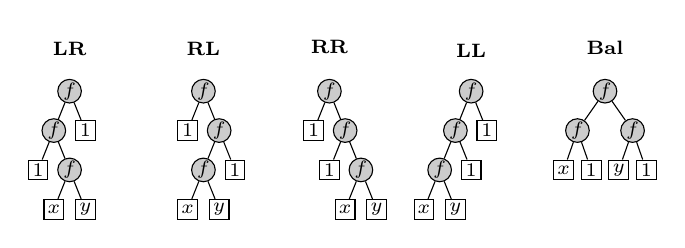
\begin{tikzpicture}[
  level distance=5mm, sibling distance=4mm,
  every node/.style={circle, draw, minimum size=3mm, inner sep=0pt, font=\scriptsize},
  active/.style={fill=black!20},
  leaf/.style={rectangle, draw, minimum size=2.5mm, font=\scriptsize},
  label/.style={draw=none, fill=none, font=\scriptsize\bfseries, minimum size=0},
]
% LR tree
\begin{scope}[xshift=0cm]
\node[label, above] at (0,0.3) {LR};
\node[active] (r) at (0,0) {$f$}
  child { node[active] {$f$}
    child { node[leaf] {1} }
    child { node[active] {$f$}
      child { node[leaf] {$x$} }
      child { node[leaf] {$y$} }
    }
  }
  child { node[leaf] {1} };
\end{scope}
% RL tree
\begin{scope}[xshift=1.7cm]
\node[label, above] at (0,0.3) {RL};
\node[active] (r) at (0,0) {$f$}
  child { node[leaf] {1} }
  child { node[active] {$f$}
    child { node[active] {$f$}
      child { node[leaf] {$x$} }
      child { node[leaf] {$y$} }
    }
    child { node[leaf] {1} }
  };
\end{scope}
% RR tree
\begin{scope}[xshift=3.3cm]
\node[label, above] at (0,0.3) {RR};
\node[active] (r) at (0,0) {$f$}
  child { node[leaf] {1} }
  child { node[active] {$f$}
    child { node[leaf] {1} }
    child { node[active] {$f$}
      child { node[leaf] {$x$} }
      child { node[leaf] {$y$} }
    }
  };
\end{scope}
% LL tree
\begin{scope}[xshift=5.1cm]
\node[label, above] at (0,0.3) {LL};
\node[active] (r) at (0,0) {$f$}
  child { node[active] {$f$}
    child { node[active] {$f$}
      child { node[leaf] {$x$} }
      child { node[leaf] {$y$} }
    }
    child { node[leaf] {1} }
  }
  child { node[leaf] {1} };
\end{scope}
% Balanced tree
\begin{scope}[xshift=6.8cm,
  level 1/.style={sibling distance=7mm},
  level 2/.style={sibling distance=3.5mm}]
\node[label, above] at (0,0.3) {Bal};
\node[active] (r) at (0,0) {$f$}
  child { node[active] {$f$}
    child { node[leaf] {$x$} }
    child { node[leaf] {1} }
  }
  child { node[active] {$f$}
    child { node[leaf] {$y$} }
    child { node[leaf] {1} }
  };
\end{scope}
\end{tikzpicture}}% end resizebox
\Description{Five depth-3 tree topologies: LR, RL, RR, LL (chains) and Balanced, showing which nodes carry active computation.  Internal nodes labeled $f$ to indicate the topology applies to any binary operator.}
\caption{Depth-3 active-subtree shapes used to generate target
expressions.  The labels LR, RL, RR, and LL describe left/right
routing of the active chain through the binary operator $f$; Bal
denotes the balanced two-branch topology.}
\label{fig:topologies}
\end{figure}

The targets used throughout are the closed forms produced by
substituting the variable leaves $\{x, y\}$ into each shape in
Fig.~\ref{fig:topologies}.  Two assignments per shape exist
($(x,y)$ and $(y,x)$), and the labels in the result tables abbreviate
them.  \emph{Paper}\,$(y,x)$ is the LR target
$\mathrm{eml}(\mathrm{eml}(1, \mathrm{eml}(y,x)), 1)$ used as the
single-leaf example in~\citep{Odrzywolek2026eml}, T1\,$(x,y)$ is the
RL target $\mathrm{eml}(1, \mathrm{eml}(\mathrm{eml}(x,y), 1))$,
T4\,$(x,y)$ is the RR target
$\mathrm{eml}(1, \mathrm{eml}(1, \mathrm{eml}(x,y)))$, and T8\,$(x,y)$
is the LR target with leaves swapped.  The yx variants apply the
$x \leftrightarrow y$ relabeling to the same shape.

%% -------------------------------------------------------------------
\subsection{Recoverability framework}
\label{sec:framework}
%% -------------------------------------------------------------------

Let $A$ denote an architecture with trainable parameters
$\Theta_A$.  These parameters are the leaf weights together with
the selector parameters at every softmax and sigmoid internal
node.  Training starts from an initial value
$\theta_0 \in \Theta_A$ drawn at random and produces a final
value $\theta_T$ by minimizing the training loss.  Each selector
is then hardened by the one-hot snap, in which every softmax and sigmoid is
replaced by the $\arg\max$ of its inputs, and branches no longer
selected are removed, leaving a concrete expression
$H(A,\theta_T)$ in closed form.

The representable set
\begin{equation}
  E(A) = \{H(A, \theta) : \theta \in \Theta_A\}
\end{equation}
collects every expression that hardening can produce.
The recoverability of a target $f^\star$ under $A$ is
\begin{equation}
  R(A, f^\star) \;=\; \Pr_{\theta_0,\,\text{train}}\bigl[\,H(A,\theta_T) \equiv f^\star\,\bigr],
  \label{eq:recover}
\end{equation}
the probability, over random initialization and the training
procedure, that the hardened expression matches $f^\star$ both
structurally and numerically.  Both
checks are necessary.  Two trees of the same shape can carry
different leaf weights and represent different functions, while
numerically close expressions need not recover the intended
symbolic structure.  Structural match compares the post-snap
tree against $f^\star$ using a canonical signature.  The
signature accounts for operator commutativity at symmetric
nodes, treats algebraically equivalent leaf compositions as
identical, and requires each leaf weight to fall within
$10^{-6}$ of its target.
Numerical match requires held-out RMSE below $10^{-6}$.  The
empirical estimator $\hat R$ averages recovery uniformly over
64 seeds and 4 initialization strategies (256 trials per
$(A, f^\star)$ pair where applicable).  Other sources of
randomness are held fixed at the defaults established by the
sensitivity check in Section~\ref{sec:setup}.

The relation $f^\star \in E(A)$ does not imply $R(A, f^\star) > 0$.
The central hypothesis tested below is that representability is
necessary but not sufficient under the tested gradient-based
training and hardening procedure.  A target may lie in $E(A)$
while still having near-zero empirical recoverability.
The remainder of the paper measures $\hat R$ across architectures,
operators, and target shapes and reports the gap between
representability and recovery.

\begin{table}[t]
\centering
\caption{Architectures studied at depth~3.}
\label{tab:archs}
\footnotesize
\begin{tabular}{@{}llrl@{}}
\toprule
Name & Internal selection & Params & Variable routing \\
\midrule
Eq.\,6 & softmax $\{1,x,f\}$ & 42 & $x$ at all nodes; $y$ at leaves \\
V16    & sigmoid $\{1,f\}$   & 38 & $x,y$ at leaves only \\
Hybrid & V16 + root 4-way    & 44 & $x,y$ at root and leaves \\
\bottomrule
\end{tabular}
\end{table}
